\documentclass{vldb}

\usepackage{graphicx}

\title{Title goes here}
\author{Filippo Sestini \\ Vrije Universiteit \\ email@host.com \and
  Davide Dal Bianco \\ Vrije Universiteit \\ email@host.com}

\begin{document}
\maketitle

\section{Introduction}
% what is this project about and why is it interesting?

\section{Related Work}
% meaningfully summarize related literature to explain what this project builds
% on, in particular, discuss the two research papers chosen with this project
% (and discussed in your presentation)

\subsection{OpenSky Network}

Most of aircraft are provided with ADB-S transmitter, which send continuosly information about the status and the position of the aircraft to guarantee better air traffic control. The messages are not encripted end, in most region, this technology will become mandatory in 2020. For these reasons OpenSky network was recently born.

OpenSky is an open source network that aggregates ADS-B messages collected by volunteers around the globe. The dataset is accessible to everyone for non-profit purposes and the data is provided in the raw format, in order to perform research and statistics about air traffic. \\
However there are some limitation to the data. Only part of Europe has a good coverage, which means there are many areas where is not yet possible to detect airplanes informations. Furthermore messages are collected by volunteers and there is not guarantee that antennas are working properly 24/7.

    \subsubsection{ADS-B messages}

    The ADS-B standard defines different kinds of messages which are sent at different frequencies:

    \begin{itemize}
        \item \textit{Aircraft identification} messages contain the callsign of the airplane;
        \item \textit{Airborne position} messages contain altitude, latititude and longitude of the airplane and are sent twice per second;
        \item \textit{Airborne velocity} messages contain climb rate and velocity of the airplane.
    \end{itemize}

    In addition to these messages, other emergencies, priority, capability, navigation accuracy category, and operational modes messages could be broadcasted.

\subsection{Routes detection}

A way to reduce the number of air routes is illustrated in \textit{J. DeArmon et al, Air Route Clustering for a Queuing Network Model of the National Airspace System}. The research showed that similar routes can be grouped to reduce the number of path between a pair of airports thus decrease air traffic congestion. The same approach could be used to detect standard routes where aircraft fly, given the departure and arrival airports. The first prototype of this model has been developed to improve the air traffic flow in the National Airspace System of the USA.

    \subsubsection{Routes distance}

    Routes are represented by an ordered list of the geographical sectors where the aircrafts transit. Prior to define the clustering algorithm, it is important to define how to measure the distance between two different routes. Since each sector is identified by a code, the string editing distance can be used to measure the distance between two different routes. The distance is therefore represented by the minimum number of operation -- insertion, deletion and replacement -- to transform Route 1 into Route 2 or vice-versa. Different weight can also be applied to different operations. The distance should not depend by the length of the routes and for this reason it is then divided by the sum of the lengths of the routes. The final result represent the percentage of difference between the routes.

    \subsubsection{Routes clustering}

    Given a distance measure for each couple of routes, it is necessary to define a clustering algorithm to group them. Many methods has been tried during the research and the \textit{Leader algorithm} showed the best results. It proceed as follows:
    \begin{enumerate}
      \item A random route is assigned as leader of a new cluster;
      \item All the other routes which distance from the leader is less than a threshold are assigned to the cluster;
      \item Repeat the steps with the remaining routes until all routes are assigned to a cluster.
    \end{enumerate}

\section{Research Questions}
% which questions is this project trying to answer, and/or hypotheses to
% investigate? These should cover both the project topic, as well as the
% technological side (aptness of the tools for the job, scalability of the
% solution).

\begin{itemize}
  \item What are the standard routes?
  \item Which flights and airlines diverge from them? In which airports?
  \item How much CO2 would be saved if aircrafts followed a straight-line route
  instead of the standard one?
\end{itemize}

Additionally

\begin{itemize}
  \item How to use raw ADS-B data to identify flights?
\end{itemize}

\section{Project Setup}
% the steps taken during the project.

\subsection{Technologies}
% spark, scala, etc
% python, haskell for scripting, etc

\subsection{Algorithm overview}

Our processing algorithm is composed of three phases that are executed in
sequence. The output of a phase is the input of the next. The process starts
from a dataset of raw ADS-B messages encoded in AVRO format, and ends producing
the data necessary to answer our research questions. The phases are the
following:

\begin{enumerate}
  \item \textbf{Position extraction}: the dataset of AVRO-encoded ADS-B messages
  is analyzed to extract only the position information abount the aircrafts. In
  particular, this phase produces a table of timestamped position points with
  latitude, longitue and altitude. Every position point is associated to a
  particular aircraft, identified by a unique ICAO code.
  \item \textbf{Flight detection}: the unstructured position points are analyzed
  per aircraft (per ICAO), and grouped together to extract single discrete
  flights. For each detected flight, departure and arrival airports are
  computed.
  \item \textbf{Route detection}: flights are grouped by pair of departure and
  arrival airport, and sent to an aggregative clustering algorithm that is used
  to identify standard routes and routes that diverge from them.
\end{enumerate}

These three phases are explained in more detail in the sections that follow.

\subsection{Positions}

Decoding the position of an aircraft from ADS-B position messages is more
complicated than one would expect. Information on latitude and longitude is
divided into two types of position messages: odd and even. Both these types of
messages are needed to correctly decode the position. This is according to a
format called Compact Position Reporting (CPR), which allows to encode higher
resolution information in less bits, but is obviously less straight-forward to
decode.

For the actual decoding in our algorithm we used the java-adsb library, which
however makes the effective parallelization of the entire operation more
challenging. In partocular, the decoding procedure implemented by the library is
essentially sequential, in that all position messages of a particular aircraft
must be submitted in order of increasing timestamp. This renders the
distribution and parallelization of the process practically impossible.

However, even though the positions for a single aircraft must be decoded
sequentially by a single node, it is still possible to distribute the data by
aircraft, allowing us to spread the work among the cluster. The distribution
involves grouping operations that are known to be particularly expensive, since
they require a lot of data to be shuffled and shared between the nodes.
Nevertheless, we did not see alternative approaches to the problem, given the
(quite intrinsic) limitations of the decoding process.

The position decoding algorithm goes through the following phases:

\begin{enumerate}
  \item Extract the raw messages and their timestamp from the avro-encoded data
  \item Decode the messages from the raw representation
  \item Filter out messages that are not position messages
  \item Order the messages according to their timestamp
  \item Group the messages by ICAO
  \item For each ICAO, go through the messages in order of timestamp and decode
  the positions
\end{enumerate}

Notice that, even if we were able to distribute the work by ICAO, there is still
a very high number of messages to be processed by a single worker node. In order
to avoid memory problems, we decided to split the decoding process between days,
therefore running the above algorithm separately for each day that we had
available in the dataset. This choice has obvious consequences on the phases
that follow, as we were not able to detect flights between two different days.
From our observations, however, we concluded that these flights are not very
frequent, so at the end of the day the final results did not suffer too much.

\subsection{Flights}

\begin{figure}[h]
  \centering
  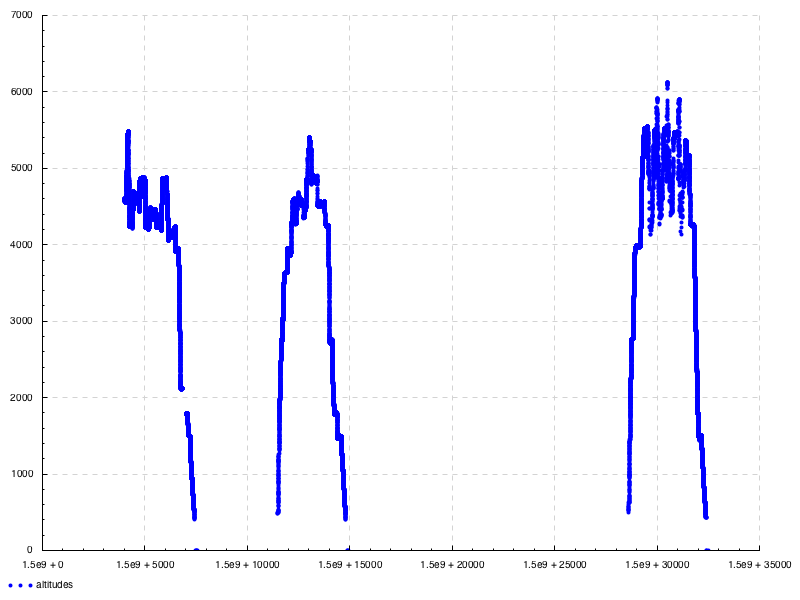
\includegraphics[scale=0.28]{imgs/4b7fad-altitudes.png}
  \caption{Altitude values of the aircraft with ICAO 4b7fad, during September
    20th, 2016. It can be seen that the data points disappear when the aircraft
    approaches the ground. Also, in the group of points of the left, the
    information on the first part of the flight is entirely missing, and the
    first point available has timestamp 06:46 am. This is almost
    certainly due to the airplane traveling through a poorly covered area.}
  \label{fig:alts}
\end{figure}

Having extracted all position information from the raw avro files, there is now
the problem of identifying discrete flights from it.
Given a sequence of positions for a given aircraft, on a particular day, we
though about how to group this information in chunks, each chunk representing a
potential flight. An important insight is given by observing the data: ADS-B
messages systematically stop being received by the sensors when the aircraft
approaches the ground. It follows that there must be a pause in the data between
two different flights, and in particular between the landing of a flight and the
take-off of another.

Another point to consider is the characteristics of position messages received
during a flight. Position messages are sent by the aircrafts several times per
minute, so two subsequent entries are likely to differ very slightly in their
space, altitude and timestamp values. If they are not, then these messages are
not considered good enough for our purposes.

Position points for a given aircraft are thus grouped together according to a
simple clustering algorithm: all points are analyzed in order of timestamp, and
two subsequent points are considered belonging in the same cluster if and only
if they are no more than 20 minutes apart, their distance is no more than 20
kilometers and their altitudes differ no more than 200 meters.

Each group is then further analyzed to determine if it actually corresponds to a
single flight or not. Again, the analysis is fairly simple, and it considers
altitude information of the points to detect take-offs and landings. In
particular, a group of points is considered a valid flight if and only if it
starts and ends with points at an altitude of 3000 m or below, and shows an
ascent as well as a descent. Ascents and descents are defined as sequences of
points which altitudes rise, respectively decrease, steadily for 2000 meters.

We acknowledge that the criteria according to which we group and filter discrete
flights are pretty restrictive, and that we inevitably throw away a lot of data
and possibly some flights in the process. However, given the unreliability of
the data and the difficult of our task, we wanted to deal with sufficiently
precise and detailed data, in order to make our life easier in the subsequent
phases of the processing. In particular, the restriction on the end points of a
flight being below 3000 m is the most important one for our purposes (as
explained below), and also the one that seems to filter out the majority of
potential flights.

\subsubsection{Departure and arrival airports}

\begin{figure}[t]
  \centering
  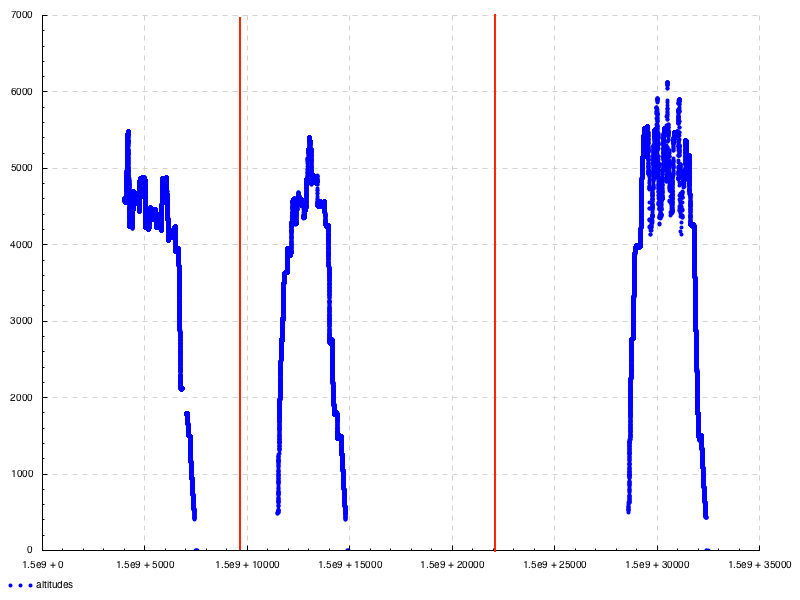
\includegraphics[scale=0.28]{imgs/4b7fad-altitudes-grouped.png}
  \caption{Altitude values of the aircraft with ICAO 4b7fad, during September
    20th, 2016, as grouped by the flight detection algorithm.}
  \label{fig:alts}
\end{figure}

A flight is given by a sequence of positions, as well as departure and arrival
airports. There two last informations, however, are not provided by the data and
must be inferred in some way. Our approach was to consider the first and last
position point of a flight, and determine the airports as the closest ones to
these points, in terms of euclidean distance.

To detect the airports, we used the help of an external dataset containing a
list of airports together with their locations. This dataset originally
contained much more data than we needed, as it also listed small non-commercial
airports. In order for our algorithm to be reasonably correct, we had to trim
the dataset first removing the airports without a IATA code, and then keeping
only commercial airports with the help of an external list we found on the
Internet. This filtering reduced the list from 6977 to 639 entries.
The resulting number of entries is still a little bit high for our purposes, but
it was nevertheless the best dataset we could get. The alternative would have
been to build a dataset by hand, which seemed extremely time consuming.

We specifically set the threshold of 3000 m in the flight detection algorithm
for purpose of airport detection: after some observations of read flights on the
website FlightRadar24, we concluded that when an aircraft goes below an altitude
of 3000 m, its position is very close to the take-off/landing airport. The
airport identification works reasonably well in this setting, and with the
external dataset. It is of couse not perfect, for two main reasons:

\begin{itemize}
  \item The dataset may still contain minor airports that are very close to
  bigger commercial ones that are the real target of a flight; in these
  situations, it is possible that the minor airport gets erroneously selected;
  \item A threshold of 3000 m may noy be sufficient in areas that contain many
  big commercial airports that are very close to each other; one example of such
  area is London.
\end{itemize}

Having considered these issues, we still settled for the simplest solution, as
we did not find alternative ways to detect airports given the data available.

\subsubsection{Sectors}

The route detection algorithm, as explained in details below, uses a
representation of flights and routes as a sequence of sectors, where each sector
represents portion of the world map. For this reason, the flights detection
phase outputs flights as sequences of sectors rather than position points. This
has two main advantages:

\begin{itemize}
  \item It prepares the data to be easily processed by the following phase of
  the algorithm
  \item It represents flights with much less space than as a highly-dense
  sequence of points
\end{itemize}

We could have considered alternative ways to eliminate redundant information and
reduce the amount of data needed to represent a single flight, but the routes
detection algorithm would stil have transformed those representations to
sequences of sectors. It follows that converting directly from position points
to sectors was obviously the best approach.

In practice, a sequence of position points is translated in a sequence of
sectors by simply truncating the latitude and longitude part of a point to one
decimal digit. Strings of values with the same truncated latitude and
longitude represent the same sector, and are compressent into one. This process
yields sectors of about 10 km by 10 km, which is a good approximation for our
purposes, where sub-kilometer precision is not needed.

\subsection{Routes}

The most important part of the process is the detection of routes between pairs
of airports. Standard routes between a pair airports are likely to be used by
the majority of flights between those airports. Our algorithm relies on the
assumption that the converse should also be true, namely that if a route is used
by the majority of flights going from an airport to another, than that route
must represent a (possibly, the) standard route between that pair of airports.

The actual route detection process relies on an aggregative clustering algorithm
that groups together flights according to a distance metric. The results of the
clustering are used to determine the standard route between a certain pair of
airports. More precisely, the algorithm goes through the following steps for
each pair of airports:

\begin{enumerate}
  \item Apply the clustering algorithm to all the flights that have the
  current pair of airports as endpoints.
  \item Select the cluster that classifies the highest number of routes.
  \item Select a route that constitues the representative of
  that cluster as the one having the least distance between al the other
  routes in the cluster
  \item The representative of this cluster determines the standard route
  between the pair of airports
  \item All the routes classified by the other clusters represent routes that
  diverge from the standard route
\end{enumerate}

The approach described above has the advantage of being simple and generally
correct in most situations. It has, of course, some problems, that come in
particular from its being fairly naive. First of all, it goes under the
assumption that the standard route, officially prescribed by the
appropriate institutions, is the one that is used by most flights. This
assumption may be invalidated in two obvious ways, among possibly others:

\begin{itemize}
  \item The analysis clearly does not take into account flights, and therefore
  routes that cannot make through the route detection phase of the algorithm.
  Our dataset is not extremely reliable, so say the least. The OpenSky Network
  has, and the time or writing this paper, a fairly good coverage of western
  Europe, but some sports may still be poorly detected by the sensors. If a
  standard route happens to pass through an area that is poorly covered, it is
  likely that other, non standard routes will be selected by the algorithm as
  standard, just because they can be detected.
  \item There may be reasons or events, such as military conflicts, for which
  airplanes are forced to systematically deviate from a standard route, for a
  period of time that can span days or even months. These temporary anomalies
  clearly invalidate this assumption, and would go absolutely undetected by our
  algorithm, especially since it gives information over just a week of time.
\end{itemize}

These, however, are fundamental problems of the data we have available. They
affect the results of the algorithm, but do not depend on it so they cannot be
reduced using a more clever algorithm. We feel that, with the information
available and in particular without an external source
of standard routes, considering this assumption as true is the best
possible approach.

However, there are some issues that have to do with the particular
implementation of the algorithm:

\begin{itemize}
  \item There could be situations where clusters have the same amount of routes,
  or the numbers differ very slightly. In this cases, the accuracy of the
  results inevitably decreases.
  \item There could be areas that are poorly covered by the sensors, or that
  have few flights passing though it. A cluster with five routes would be
  selected against one with two or three, but clearly it does not have a strong
  argument in determining the standard route between two airports. There are two
  possible approaches to this. The first is to recognize that the informations
  available is not enough, and possibly leave some pairs of airports with
  undetermined standard routes. The other, and the one that we follow, is to
  just run the algorithm without taking into account how many routes are
  actually involved in the selection of the standard route. A possible
  refinement could be to add to the front-end visualization of the standard
  routes an indication of ``accuracy'' of a particular route based on the amount
  of data available in the detection.
\end{itemize}

\subsubsection{Clustering algorithm}

Routes, both standard and nonstandard, are determined separately for each
ordered pair of airports. The pairs are ordered in the sense that routes from
Schiphol to Charles de Gaulle and Charles de Gaulle to Schiphol are considered
separately. The algorithm proceeds by grouping together flights for each pair of
airports. Then, given a particular pair, the following sequence of steps is
executed for each flight, one after the other.

\begin{itemize}
  \item Test the flight agains every already present cluster, where the test is
  positive if and only if the distance between the current flight and every
  flight in the cluster is below a certain threshold
  \item If the test is positive for some cluster, add the flight to that cluster
  \item Otherwise, create a new cluster with the current flight as the only
  classified flight
\end{itemize}

As it can be seen, the clustering algorithm proceeds by maintaining a list of
clusters that gets updated at each iteration, making it fundamentally
sequential. It follows that, on a large scale implementation, every execution of
the clustering algorithm will be carried on by a single worker. The
parallelization of the process, however, is not damaged: a separate clustering
algorithm must be executed for each pair of airports, so it sufficies to
distribute the data among the nodes by pair of airports.

Our approach of clustering together routes represented as sequences of sectors
is inspired by the Leader Algorithm described in [reference], but differs from
it in some ways. Sectors in [reference] are bounded airspace regions under the
control of a single air traffic controller or small team, hence they cover a
relatively large area. Flights with such subdivision usually go through 5--10
sectors. Our sectors are smaller --- each flight has approximately 20--40 of
them --- therefore they represent a much more fine-grained subdivision of the
world map.

In [reference], distance between two routes is computed as a simple editing
distance between a lexical representation of routes. With smaller sectors,
however, comes the need to take other factors into account. An extreme example
of why this is needed is given by two routes that are almost parallel and at
distance of slightly more than 10 km. In our subdivision in sectors of 10 km by
10 km, these two routes would end up represented by a sequence with almost no
common sectors, even though they are actually very similar. A simple editing
distance function would assign the same value to this pair of routes, as well as
another pair of routes much more distant and different from each other.

To avoid errors in the clustering, we also consider the euclidean distance
between differing sectors of two routes as a weight in the final result. This
values, together with the editing distance, determine the distance between two
routes. The threshold at the heart of the algorithm, as well as the other
parameters, have been fine-tuned with experimentations and
observation of the results.

To aid the visualization, we consider ``diverging clusters'' instead of
diverging flights. After the clustering process, all clusters different from the
one selected as standard are diverging clusters. We then display the
representatives of the diverging clusters as the diverging routes for each
airport. The rationale is simply that routes in the same cluster are close
enough to be abstracted by a single representative of the entire group.

\subsubsection{CO2 consumption}

\begin{figure}[t]
  \centering
  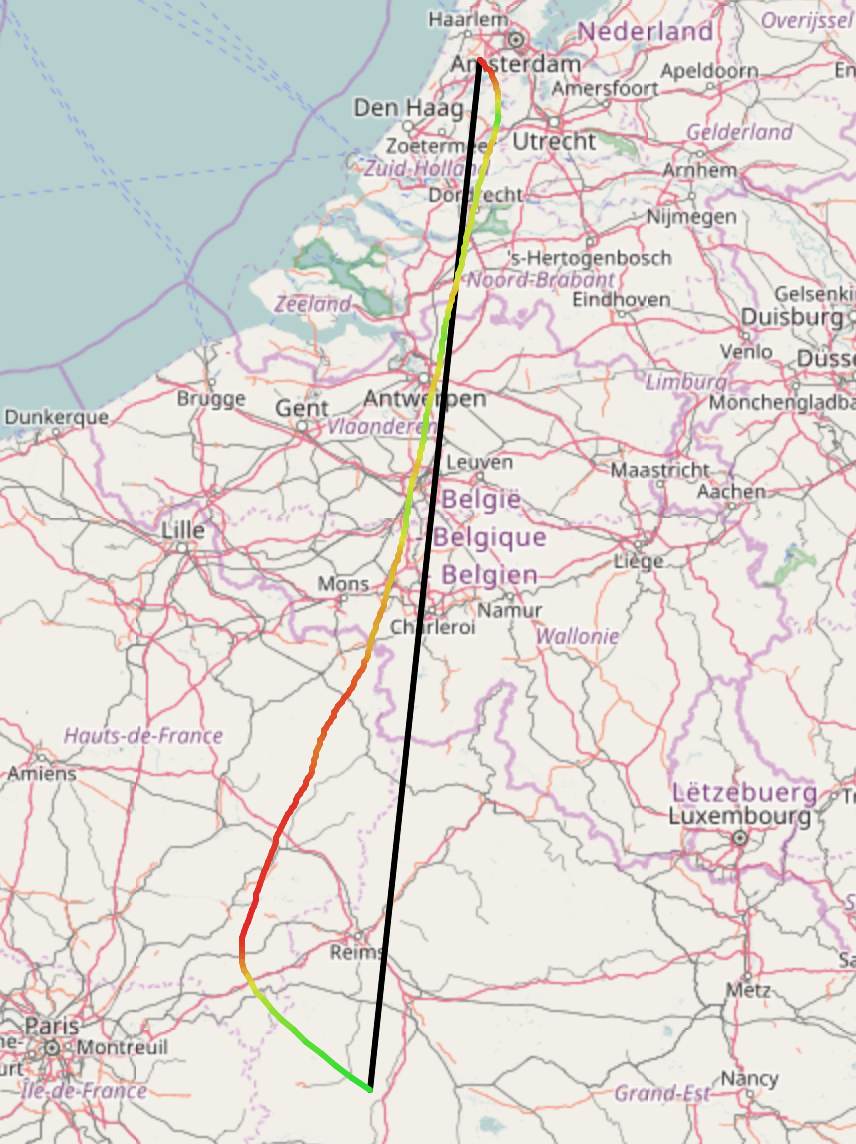
\includegraphics[scale=0.4]{imgs/amsterdam-vatry-co2.png}
  \caption{Visualization of CO2 consumption for the standard route from
    Amsterdam to Vatry. It can be seen that the route is mostly green for the
    first part. It then shifts to red in the last part, where it takes a detour
    from the straight-line route.}
  \label{fig:amsterdam-vatry}
\end{figure}

A little research showed that an average aircraft procudes about 53 pounds of
carbon dioxide per mile. We used this value to compute the difference in CO2
production between the standard routes and the corresponding straight-line
route.

We also wanted to offer a visualization of the comsumption of fuel with respect
to a straight-line route. The visualization should show the points of a given
route on the map in different colors on a palette from greed to red, where hues
towards red would indicate a point of high consumption in the route.
To do this, we needed to attribute to each segment of the route a suitable value,
from which we could determine its color. Rather than trying to compute a value
of ``comsumption'' for each segment, we decided to determine it based on
how different the route is with respect to the straight-line route. The main
characteristic of a straight-line route is that the airplane always points to
the destination airport. Therefore, we considered as value of each segment the
angle between the direction that the aircraft is facing in that segment and the
direction of the destination airport. Higher values lead to more red segments.

\subsection{Deployment on the hadoop cluster}
% how we actually implemented the algorithms on the hadoop cluster

When working of large-scale datasets, it is essential to understand the
available data and try to extract only relevant information from it. The
subdivision of our algorithm in different phases is not only a convenient
logical partitioning of operations, but it is essential to transform the dataset
into smaller datasets, tailored to our needs. It is useful to do this
transformation gradually, step by step, so that single intermediate phases can
be reiterated without affecting the previous ones.

The whole algorithm has been implemented as a Scala + Spark project, that has
been deployed to the Hadoop cluster. We developed every phase of the algorithm
as a separate executable Scala class, allowing us to run each phase separately.

The position extraction phase was run on the entire dataset of raw AVRO-encoded
messages, and it was, and one could expect, the most time consuming. The entire
execution took about 48 hours. As a result of this phase, we were able to shrink
the data from about 85 GB per day to about 10 GB of position points per day.
This of course made the next phases of the algorithm more tractable. Position
data has then been processed by the flight detection algorithm, in about 24
hours. This phase, as we already explained, throws away a lot of data. Also,
flights are represented and saved to disk as sequences of sectors, where each
flight it composed of 20--50 sectors. This gives a very succint representation,
and we were able to store the output of this phase in just about 4 MB per day.
The small size of the flights data allowed us to run the route clustering
algorithm and all the additional JSON files generation for the visualization in
under 30 minutes. With such small execution time, we were able to test the
results of the algorithm several times, and improve its performance and results.

\section{Experiments}
% a description of the experiments and their results.

\begin{figure}[t]
  \centering
  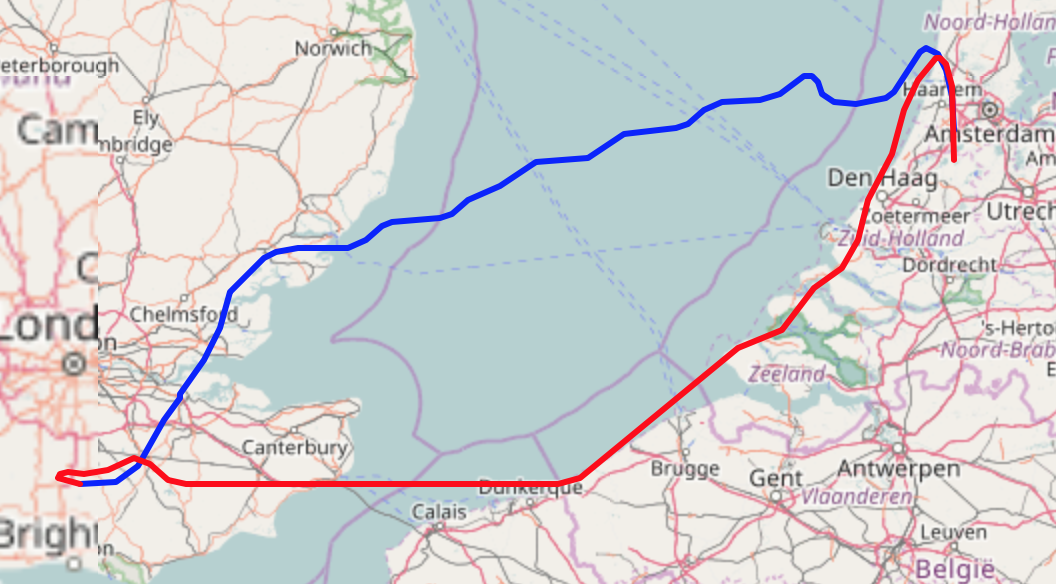
\includegraphics[scale=0.4]{imgs/gatwick-schiphol.png}
  \caption{Results of standard (blue) and diverging (red) routes detection for
    flights from London Gatwick to Amsterdam Schiphol.}
  \label{fig:gatwick-schiphol}
\end{figure}

\paragraph{Flight detection}

We carried out some experiments on the results of the various phases and
algorithms, in order to asses their behaviour. Some statistic data collected in
the flight detection phase show how our classification criteria turned out to be
pretty restrictive, as expected.

This result should be attributed to the restrictive criteria of the
classification algorithm, as well as to the incomplete information provided by
the dataset. It should be recalled that, even though the OpenSky network
comprises at the moment of 70 active sensors, some spots in the western Europe
area may still be pooly covered, or not covered at all. Even a small poorly
covered are makes all information on the flights passing through it incomplete,
thus unsuitable for our analysis.

It should also be considered that what our algorithm considers as a cluster is
just a group of position points that is sufficiently dense. A cluster does not
necessarily corresponds to a flight with incomplete data (and most of the times
it doesn't). Comparing the number of detected flights with the total number of
clusters is not a good indication of the undetected flights or the amound of
position points discarded by the algorithm.
Having said this, the table still gives an idea of how good the dataset is. In
an ideal dataset, every cluster corresponds to a flight.

% TODO make a table
%%% position grouping
% LOG: positions-20160918 has 199030 clusters and 1219 flights
% LOG: positions-20160919 has 170594 clusters and 1103 flights
% LOG: positions-20160920 has 126370 clusters and 1241 flights
% LOG: positions-20160921 has 127855 clusters and 1205 flights
% LOG: positions-20160922 has 127982 clusters and 1308 flights
% LOG: positions-20160923 has 130662 clusters and 1243 flights
% LOG: positions-20160924 has 121624 clusters and 874 flights

\paragraph{Airlines}

In order to compute the amount of flights diverging from a standard route per
airline, we needed to associate a an airline to each flight. This is not a
completely trivial task, as airline information is not provided at all by the
data. Every aircraft, hence every flight, has an ICAO number associated to it,
from which it is possible to determine callsigns from the identification
messages in the dataset. In the case of commercial flights, the callsign of an
aircraft contains the ICAO three-letter code of the airline for which the
vehicle is flying for at the moment. Since aircraft are bought by airlines and
hardly transferred from an airline to another, it is safe to assume that only
one callsign is sufficient to determine the airline of an aircraft.
The mapping between three-letter ICAO codes of airlines and their name has been
done with the help of an external dataset.

Of 19860 distinct icaos for which identification messages were available, 15911
had a unique three-letter airline code in their callsigns, and 15691 had a code
actually corresponding to an airline in the dataset. The remaining 4169
icaos without a proper airline code are likely to correspond to private airplanes.

\paragraph{Diverging flights}


%%% nondiverging vs diverging flights



\section{Conclusion}
% revisit the research questions and hypotheses and try to answer them. Any new
% questions? Insights in the usability of the employed technology for particular
% tasks?

\begin{figure}[t]
  \centering
  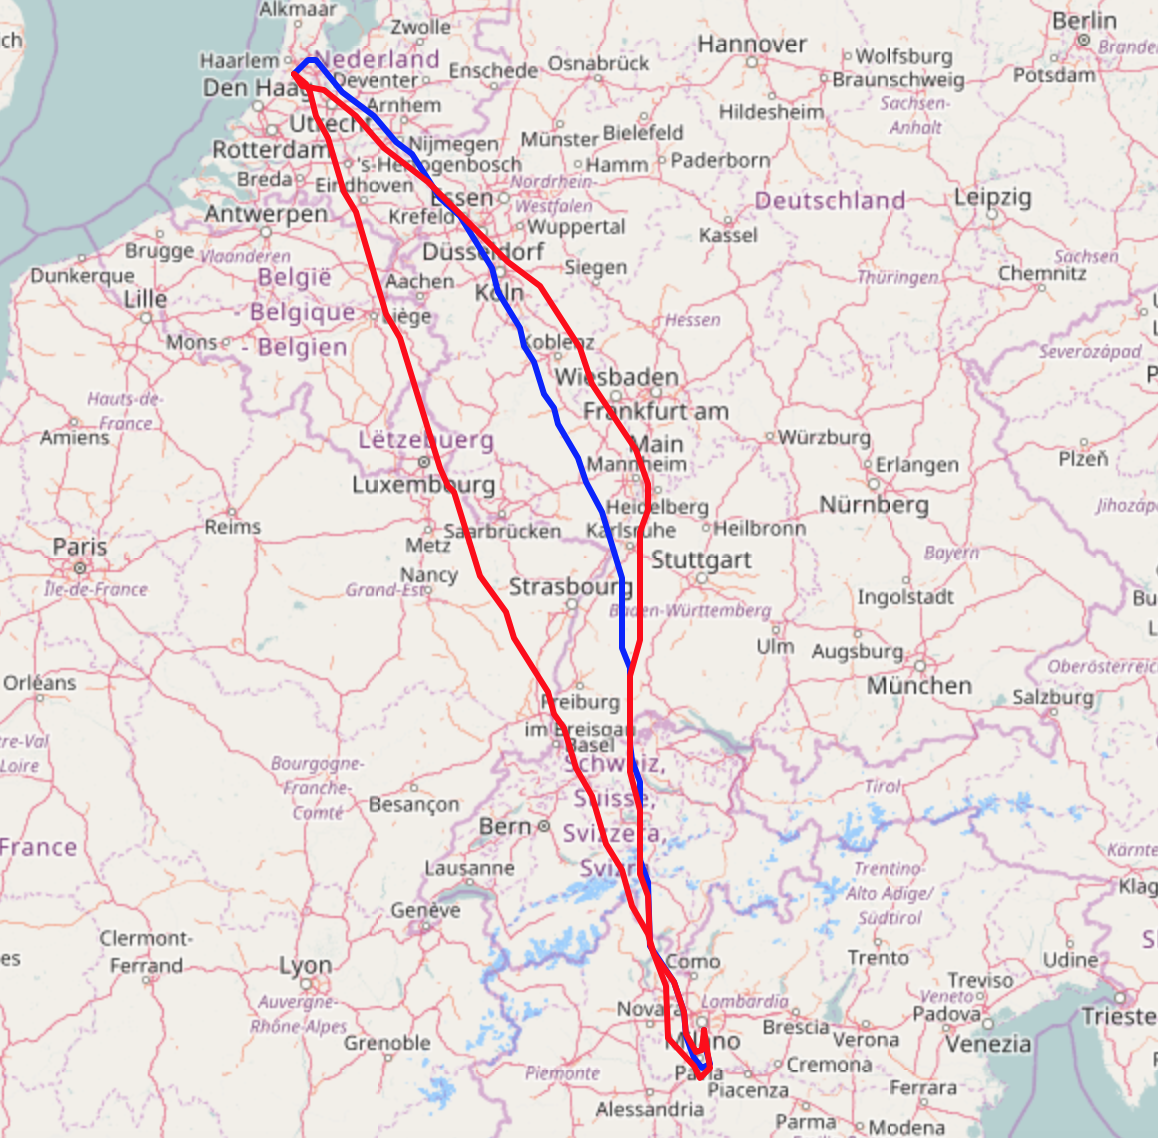
\includegraphics[scale=0.35]{imgs/schiphol-linate.png}
  \caption{Results of standard (blue) and diverging (red) routes detection for
    flights from Amsterdam Schiphol to Milano Linate. It can be seen that the
    diverging route on the right is very similar to the standard route, but the
    clustering algorithm fails to classify it as such.}
  \label{fig:schiphol-linate}
\end{figure}

... The OpenSky network counts 70 active sensors at the time of development,
yielding a pretty good coverage of the western Europe area. Some areas are
covered almost perfectly, and for those we were able to detect flight accurately.

The results from the complete execution of the algorithm are mixed.
It should be considered that there are a lot of minor airports, and flight
information for those airports is, as one could expect, incomplete.
Of 1165 of the total combinations of airports, about 85 \% of them has their
standard route determined by under 10 flights. These pairs usually correspond
to minor airports, and the accuracy of the computed standard route has
necessarily to be considered pretty low. For major airports, however, the
available data rises significantly. As an example, the standard route between
Schiphol and London Gatwick and converse has been determined by 39,
respectively 42 routes.

Tuning the distance function for the route clustering phase was more challanging
than we expected. In many cases, the algorithm ended up considering as diverging
routes that were actually very close to the standard one. We can conclude,
therefore, that even though we think we were able to determine standard routes
with acceptable accuracy and confidence for medium to big airports, diverging
routes detection still has some issues. We do think that the approach of using
sectors and editing distance can give good results in this context, but the
distance function obviously needs much more experiments are fine-tuning to be
able to give good results in all situations.

Observing our results, we conclude that it is definitely possible to
identify flights with acceptable reliability using raw ADS-B data alone. There
are however some issues with the data that make this effort less than
trivial, and some advanced techniques as well as other data sources may be
needed to determine them with more than average accuracy.

\section{Future work}

We find that the accuracy of many of our algorithms is difficult to assess,
given the lack of reliable data to compare against. Future work on this project
could start by retrieving and using such external data, when available. The most
significant effort would be to asses the correctness of the route clustering
algorithm with a precompiled dataset of standard routes.

The next step would be to improve the algorithms, by making them more clever and
use more data from the dataset in a better way. A trivial but effective
improvement to all phases of the algorithm follows, clearly, from increasing
the number of flights available to them.

The flight detection algorithm could be improved by using an external dataset
relating callsigns, which are amost fully available from the data, to flights.
At the time of writing we are not aware of such dataset being publicly
available, but there could be in the future. Also, our flight detection
algorithm does not take velocity messages into account. Velocity information is
not vital in flights detection, but we do not exclude that the heading
information of an aircraft could be combined with its altitude information to
better recognize ascents and descents. The grouping criteria in our flight
detection are quite restrictive, to be able to get sufficiently reliable outputs
with a relatively simple algorithm. These criteria can surely be made less
restrictive, using some more advanced techniques to make up for missing points.

There is room for improvement in the route detection algorithm, for example
by tuning the way routes are clustered together, and in particular by selecting
a better distance function.
A possible alternative way to compute the distance could be to compute the area
delimited by two routes. This area, normalized according to the length of the
routes, could be a good estimate of how ``different'' two routes are.
A different approach could be to discard the current algorithm and instead use
an external dataset of standard routes. In this setting, standard routes need
not be computed. Flights that diverge from them can simply be discovered by
computing the distance from the standard route for the particular pair of
airports, and checking the result against a threshold.

Currently, the CO2 consumption for the flights is computed in a very simple way,
by multiplying the distance traveled by the airplanes by an estimate of the
quantity of CO2 that an average aircraft produces per mile. A better approach
could use the ICAO number of each single aircraft to index an external dataset
and discover its characteristics. These properties could be used to compute a
more precise and realistic estimate of CO2 production.

% TODO: How other work could be based on ours?

\end{document}